\begin{center}
    \begin{tikzpicture}
        % 定义正三角形的边长
        \def\sideLength{3}

        % 定义点
        \coordinate (A) at (0,0);
        \coordinate (B) at (\sideLength,0);
        \coordinate (C) at (\sideLength/2,{sqrt(3)*\sideLength/2});
        % 计算 AB 的中点
        \coordinate (H) at ($(A)!0.5!(B)$);

        % 绘制正三角形
        \draw (A) -- (B) -- (C) -- cycle;
        \draw[dashed] (C) -- (H);

        % 标记顶点
        \node[below left] at (A) {$A$};
        \node[below right] at (B) {$B$};
        \node[above] at (C) {$C$};
        \node[below] at (H) {$H$};
        \draw[decorate,decoration={calligraphic brace,amplitude=3mm,raise=2pt},ultra thick] (C) -- (B); 
        %raise 表示让括号位移一点 amplitude 控制花括号的弯度程度 
        % calligraphic brace 有粗细变换的括号
        \node at ($(C)!0.5!(B)$) [above=8pt,right=8pt] {$x$};
    \end{tikzpicture}
\end{center}

一个正三角形的边长为$x$,则其高为$\frac{\sqrt{3}}{2} x$, 则其面积为 $\frac{\sqrt{3}}{4} x^2$.

\begin{center}
    \begin{tikzpicture}[scale=2]
        % 定义正六边形外接圆半径
        \def\radius{1}
        % 定义正六边形顶点坐标
        \coordinate (A) at (\radius, 0);
        \coordinate (B) at ({0.5 * \radius}, {sqrt(3) * 0.5 * \radius});
        \coordinate (C) at ({-0.5 * \radius}, {sqrt(3) * 0.5 * \radius});
        \coordinate (D) at (-\radius, 0);
        \coordinate (E) at ({-0.5 * \radius}, {-sqrt(3) * 0.5 * \radius});
        \coordinate (F) at ({0.5 * \radius}, {-sqrt(3) * 0.5 * \radius});

        % % 绘制顶点
        % \foreach \point in {A, B, C, D, E, F} {
        %     \fill (\point) circle (2pt);
        % }

        % 绘制正六边形的边
        \draw (A) -- (B) -- (C) -- (D) -- (E) -- (F) -- cycle;
        \draw[dashed,line width=0.2pt] (A)  -- (D) ;
        \draw[dashed,line width=0.2pt] (B)  -- (E) ;
        \draw[dashed,line width=0.2pt] (C)  -- (F) ;

        % % 标记顶点
        % \foreach \point in {A, B, C, D, E, F} {
        %     \node[above right] at (\point) {$\point$};
        % }

        \draw[decorate,decoration={calligraphic brace,amplitude=3mm,raise=2pt},ultra thick] (B) -- (A); 
        \node at ($(A)!0.5!(B)$) [above=8pt,right=8pt] {$x$};
    \end{tikzpicture}
\end{center}


因为一个正六边形能分割成$6$个全等的正三角形,所以边长为$x$的正六边形的面积是 $6 \times \frac{\sqrt{3}}{4} x^2  $.






\begin{figure}[H]
    \centering
	\begin{tikzpicture}[scale=1.5]
    % 定义正三角形的边长
    \def\sideLength{3}
    % 定义点
    \coordinate (A) at (0,0);
    \coordinate (B) at (\sideLength,0);
    \coordinate (C) at (\sideLength/2,{sqrt(3)*\sideLength/2});
    % 计算 AB 的中点
    \coordinate (H) at ($(A)!0.5!(B)$);
    \coordinate (O) at ($(H)!0.3333!(C)$); % 中点

    %填涂区域
    \fill[blue!20] (A) -- (O) -- (H) -- cycle;




    % 绘制正三角形
    \draw (A) -- (B) -- (C) -- cycle;
    % \draw[dashed] (C) -- (H);
    \draw[dashed,ultra thick, red] (C) -- (O);
    \draw[dashed,ultra thick,blue] (O) -- (H);
    % \draw[dashed,thick,blue] (C) -- (O);
    \draw[dashed] (A) -- ($(C)!0.5!(B)$);
    \draw[dashed] (B) -- ($(C)!0.5!(A)$);


    % 标记顶点
    \node[below left] at (A) {$A$};
    \node[below right] at (B) {$B$};
    \node[above] at (C) {$C$};
    \node[above=5pt,right] at (H) {$H$};
    \node[right=3pt,red] at (O) {$O$};

    \fill (O) circle (2pt);%填涂测试
\end{tikzpicture}

\end{figure}
一个正三角形还能被分割成如图所示的$6$个全等的直角三角形,则线段 $|CO|$ 与线段 $|OH|$ 的比值为 $2$\footnote{你能证明吗?}.

\subsection{弧度制的复习}
扇形是由圆心角的两条半径和圆心角所对的弧围成的图形。在研究扇形时,常用到以下参数:
\begin{itemize}
    \item 半径:用 \( r \) 表示,即扇形两条边的长度。
    \item 圆心角:用 \( \theta \) 表示(通常使用弧度制),它决定了扇形的张开程度。
    \item 弧长:用 \( l \) 表示,根据弧度制的定义,弧长与半径和圆心角的关系为 \( l = r\theta \)。
\end{itemize}


\begin{figure}[h]
    \centering
    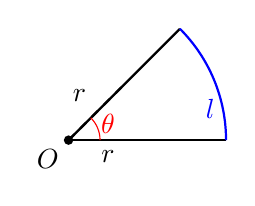
\begin{tikzpicture}[scale=2]
        % 绘制扇形
        \draw[thick] (0,0) -- (1,0);
        \draw[thick] (0,0) -- (0.707,0.707);
        \draw[thick,blue] (1,0) arc (0:45:1);
        
        % 标注
        \draw[thick,dashed] (0,0) -- (0.5,0) node[midway,below]{\( r \)};
        \draw[thick,dashed] (0,0) -- (0.3535,0.3535) node[midway,above left]{\( r \)};
        \draw[red] (0.2,0) arc (0:45:0.2);
        \node[red] at (0.25,0.1) {\( \theta \)};
        \node[blue] at (0.9,0.2) {\( l \)};
        
        % 圆心
        \fill[black] (0,0) circle (0.03);
        \node[below left] at (0,0) {\( O \)};
    \end{tikzpicture}
    \caption{扇形的基本参数示意图}
\end{figure}




比例法推导扇形面积公式的核心思路是利用扇形面积与整个圆面积的比例关系,该比例等于扇形圆心角与整个圆周角的比例。推导步骤如下:
\begin{enumerate}
    \item 我们知道圆的面积公式为 \( S_{\text{圆}} = \pi r^2 \),这是基于圆的定义和数学推导得出的。
    \item 因为整个圆周角为 \( 2\pi \)(弧度制),而扇形的圆心角为 \( \theta \),所以扇形圆心角 \( \theta \) 占整个圆周角 \( 2\pi \) 的比例为 \( \frac{\theta}{2\pi} \)。
    \item 由于扇形面积 \( S \) 与圆面积 \( S_{\text{圆}} \) 的比例和圆心角的比例相同,那么扇形面积 \( S \) 就可以表示为 \( S = \frac{\theta}{2\pi} \times \pi r^2 \)。
    \item 对上式进行化简,\( S = \frac{\theta}{2\pi} \times \pi r^2=\frac{1}{2} r^2 \theta \),这样我们就得到了扇形面积公式。
\end{enumerate}

为了更直观地理解,我们可以参考图 \ref{fig:ratio_method},该图展示了圆与扇形的关系。

\begin{figure}[h]
    \centering
    \begin{tikzpicture}[scale=1.5]
        % 绘制圆
        \draw[thick] (0,0) circle (1);
        
        % 绘制扇形
        \fill[blue!20] (0,0) -- (1,0) arc (0:120:1) -- cycle;
        \draw[thick] (0,0) -- (1,0);
        \draw[thick] (0,0) -- (-0.5,0.866);
        \draw[thick,blue] (1,0) arc (0:120:1);
        
        % 标注
        \draw[red] (0.3,0) arc (0:120:0.3);
        \node[red] at (0.3,0.3) {\( \theta \)};
        \node at (0.3,0.6) {\( S \)};
        \node[below] at (0,-1.2) {\( S_{\text{圆}} = \pi r^2 \)};
    \end{tikzpicture}
    \caption{比例法推导扇形面积公式示意图}
    \label{fig:ratio_method}
\end{figure}

